\subsection{Convergence Study}

Figure~\ref{fig:sample-subfig} compares two configurations side by side. \lipsum[14]

% Sub-figure pair: each panel carries its own caption and label.
\begin{figure}[ht!]
    \centering
    \begin{subfigure}{0.48\textwidth}
        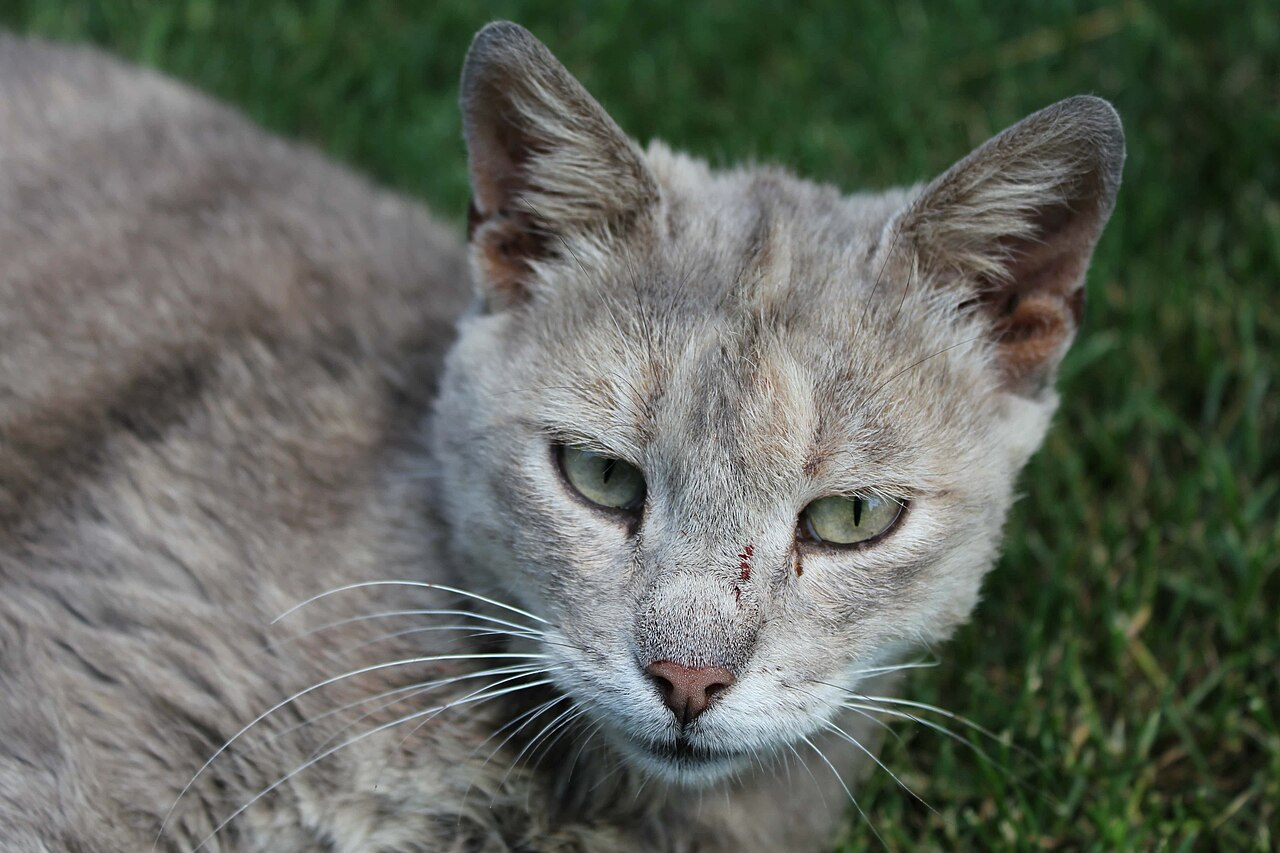
\includegraphics[width=\textwidth]{Diagram/sample-cat.jpg}
        \caption{Configuration A.}
        \label{fig:sample-subfig-a}
    \end{subfigure}
    \hfill
    \begin{subfigure}{0.48\textwidth}
        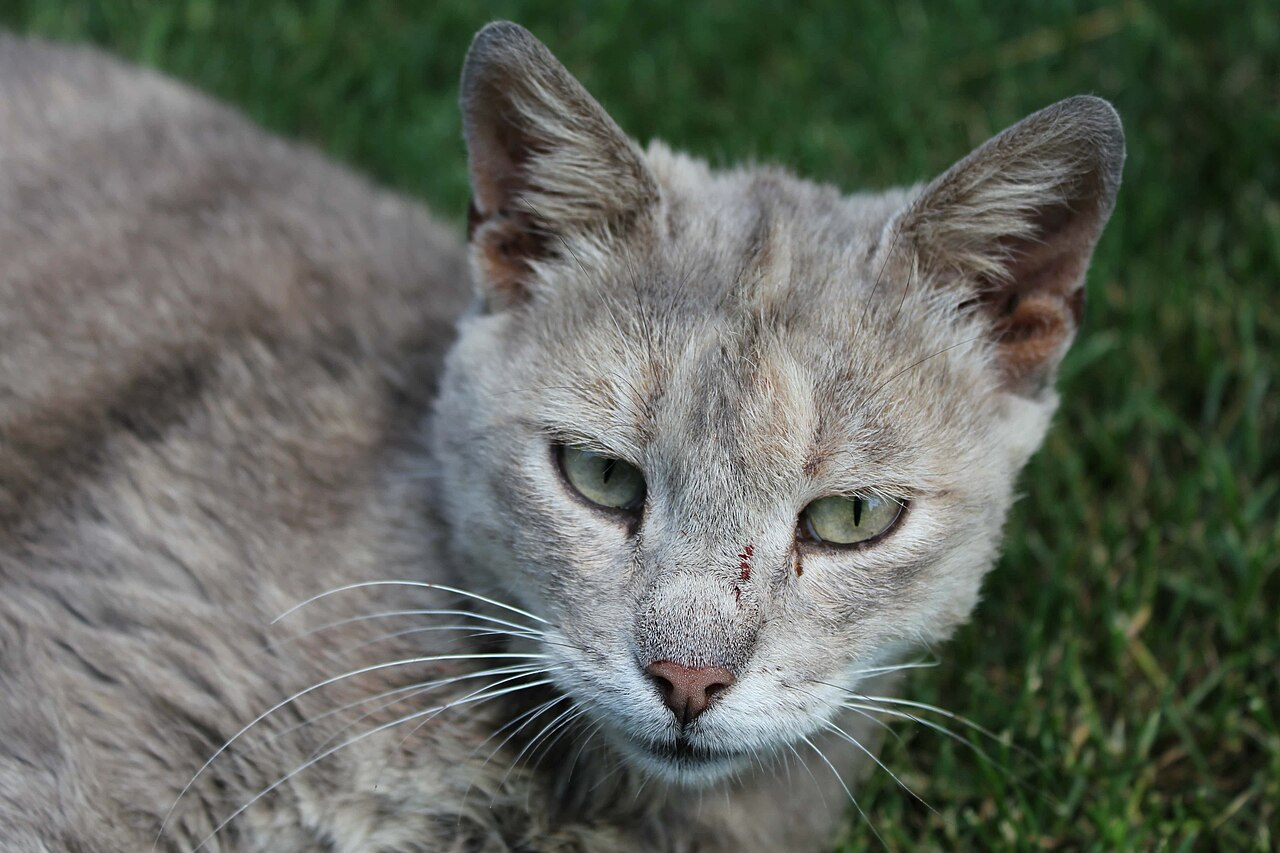
\includegraphics[width=\textwidth]{Diagram/sample-cat.jpg}
        \caption{Configuration B.}
        \label{fig:sample-subfig-b}
    \end{subfigure}
    \caption{Two sub-figures sharing one caption. \subref{fig:sample-subfig-a} and \subref{fig:sample-subfig-b} are referenced individually in the text.}
    \label{fig:sample-subfig}
\end{figure}

\lipsum[15]

\subsection{Discussion}

\lipsum[16]
